
\documentclass[compress]{beamer}
\usefonttheme{professionalfonts}



%

\usepackage[T1]{fontenc}
%\usepackage{kmath,kerkis}
%\usepackage{fouriernc}
\usepackage[adobe-utopia]{mathdesign}
%\usepackage{arev}
\usepackage{times}
\usepackage{natbib}

\usepackage[noend]{algpseudocode}
\usepackage{xmpmulti}
\usepackage{dsfont}
\usepackage{amsmath}

\usepackage{graphicx,float,wrapfig, bbm}
\usepackage{amsfonts, comment, bbold}
\usepackage{mdwlist}
\usepackage{subfigure}
\usepackage{colortbl}
\usepackage{mathrsfs}


\usepackage{multirow}




% packages

\usepackage{amsfonts}

% environments

\newenvironment{packed_enumerate}{
  \begin{enumerate}
    \setlength{\topsep}{0pt}
    \setlength{\itemsep}{2pt}
    \setlength{\parskip}{0pt}
    \setlength{\parsep}{0pt}
}{\end{enumerate}}

\newenvironment{stepit}
 {\begin{itemize}[<+-|alert@+>]}
   {\end{itemize}}

% commands

\newcommand{\Norm}[3]{\mathcal{N}\left( #1, #2, #3 \right)}
\newcommand{\popshow}[2]{\only<#1->{\alert<#1>{#2}}}
\newcommand{\x}{\mathbf{x}}
\newcommand{\ex}[1]{\mbox{exp}\left\{ #1\right\} }
\newcommand{\e}[2]{\mathbb{E}_{#1}\left[ #2 \right] }
\newcommand{\g}{\, | \,}
\newcommand{\indpt}{\protect\mathpalette{\protect\independenT}{\perp}}
\def\independenT#1#2{\mathrel{\rlap{$#1#2$}\mkern2mu{#1#2}}}
\newcommand{\E}{\textrm{E}}
\newcommand{\R}{\textrm{R}}
\newcommand{\realline}{\mathbb{R}}
\newcommand{\data}{{\cal D}}
\newcommand{\loglik}{{\cal L}}
\newcommand{\grad}[2]{ \frac{\partial{#1}}{\partial#2}}
\newcommand{\dir}[1]{\mbox{Dir}(#1)}
\newcommand{\mult}[1]{\mbox{Mult}( #1)}
\newcommand{\G}[1]{\Gamma \left( \textstyle #1 \right)}
\newcommand{\ind}[1]{\mathds{1}\left[ #1 \right] }
\newcommand{\norm}[1]{\left\lVert#1\right\rVert}

\newcommand{\class}[1]{ \texttt{#1}}
\newcommand{\term}[1]{ ``#1''}
\newcommand{\tcword}[0]{ w }
\newcommand{\docsetlabeled}[0]{ D }
\newcommand{\onedoclabeled}[0]{ d }
\newcommand{\tcposindex}[0]{ i }
\newcommand{\myblue}[1]{ {\textbf #1 }}
\newcommand{\dnrm}[1]{ _{\mbox{\textsc{ #1 }}}}
\newcommand{\argmax}[0]{ \arg \max }
\newcommand{\tcjclass}[0]{c_j}
\newcommand{\maths}[1]{ {\bf #1}}




% complexity
\renewcommand{\O}{\mathcal{O}}



\setbeamersize{text margin left=0.5cm}
\setbeamersize{text margin right=0.5cm}
\setbeamercolor{alert}{fg=red!75!black}

\usetheme{default}
\useinnertheme{circles}
\useoutertheme{split}
\usecolortheme{seahorse}
% \usecolortheme{dove}
% \usecolortheme{seagull}
%\usecolortheme{default}
% \usecolortheme{dolphin}
\usefonttheme{structurebold}
%\usefonttheme{serif}

\setbeamertemplate{navigation symbols}{}
\setbeamertemplate{headline}{}
\setbeamertemplate{footline}{}
\setbeamerfont{itemize/enumerate subbody}{size=\normalsize}
\setbeamerfont{itemize/enumerate subsubbody}{size=\normalsize}
\setbeamercolor{itemize item}{fg=gray}
\setbeamercolor{enumerate item}{fg=gray}
\setbeamercolor{itemize item}{fg=gray}
\setbeamercolor{itemize subitem}{fg=gray}
\setbeamercolor{item projected}{bg=gray}
\setbeamercolor{subitem projected}{bg=gray}


\newenvironment{bullets}
{\begin{itemize} \setlength{\itemsep}{10pt}}
{\end{itemize}}

\newcommand{\mygraphic}[2]{
  \begin{beamercolorbox}[colorsep*=4pt]{black math}
    \begin{center}
      \includegraphics[#1]{#2}
    \end{center}
  \end{beamercolorbox}
}

\setbeamercolor{structure}{bg=gray}
\setbeamercolor{section in head/foot}{bg=gray}
\setbeamercolor{palette primary}{bg=lightgray}


\usepackage{minted}

\usetheme[pageofpages=of,                    % String used between the current page and the
                                             % total page count.
          bullet=circle,                     % Use circles instead of squares for bullets.
          titleline=true,                    % Show a line below the frame title.
          showdate=true,                     % show the date on the title page
          alternativetitlepage=true,         % Use the fancy title page.
          titlepagelogo=../../common/culogo,              % Logo for the first page.
          % Logo for the header on first page.
          headerlogo=../../common/boulder_cs,
          ]{UCBoulder}

\usecolortheme{ucdblack}
\author{Introduction to Data Science Algorithms}


\institute[Boyd-Graber and Paul] % (optional, but mostly needed)
{Jordan Boyd-Graber and Michael Paul}


\AtBeginSection[] % "Beamer, do the following at the start of every section"
{ \begin{frame} \frametitle{Outline} % make a frame titled "Outline"
\tableofcontents[currentsection] % show TOC and highlight current section
\end{frame} }
\usepackage{tikz}

\newcommand{\gfx}[2]{
\begin{center}
	\includegraphics[width=#2\linewidth]{lm/#1}
\end{center}
}
\title{Language Models}
\date{Knesser-Ney and Bayesian Nonparametrics}

\newcommand{\mymk}[2]{%
  \tikz[baseline=(char.base)]\node[anchor=south west, draw,rectangle, rounded corners, inner sep=2pt, minimum size=7mm,
    text height=2mm](char){\texttt{#1}} ;\textsuperscript{#2}}


\begin{document}


\frame{\titlepage
}



\begin{frame}{Intuition}

  \begin{itemize}
    \item Some words are ``sticky''
    \item ``San Francisco'' is very common (high ungram)
    \item But Francisco only appears after one word
      \pause
     \item Our goal: to tell a statistical story of bay area
       restaurants to account for this phenomenon
  \end{itemize}

\end{frame}


\begin{frame}{Let's remember what a language model is}
	\begin{itemize}
		\item It is a distribution over the \emph{next word} in a sentence
		\item Given the previous $n-1$ words
		\pause
		\item The challenge: backoff and sparsity
	\end{itemize}
\end{frame}

\begin{frame}{The Chinese Restaurant as a Distribution}

	To generate a word, you first sit down at a table.  You sit down at a table proportional to the number of people sitting at the table.
	\begin{center}
	\begin{tabular}{ccc}
	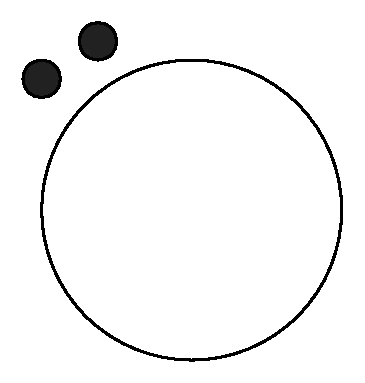
\includegraphics[width=.2\linewidth]{lm/table_2} &
	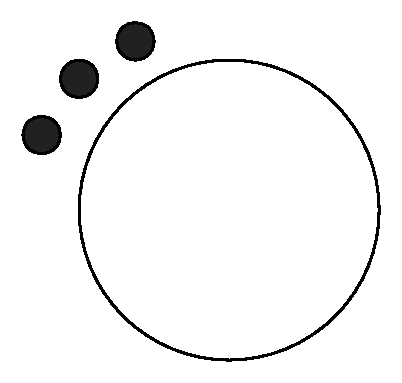
\includegraphics[width=.2\linewidth]{lm/table_3} &
         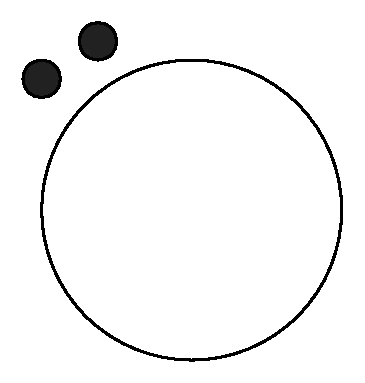
\includegraphics[width=.2\linewidth]{lm/table_2} \\
	 \pause
	 $\frac{2}{7}$ & $\frac{3}{7}$ & \alert<3->{$\frac{2}{7}$} \\
	 \pause
	 \pause
	 dog & cat & \alert<4>{purple} \\
	\end{tabular}
	\pause
	\begin{block}{But this is just Maximum Likelihood}
		Why are we talking about Chinese Restaurants?
	\end{block}
	\end{center}

\end{frame}

\begin{frame}{Always one more table \dots}

	\begin{center}
	\begin{tabular}{cccc}
	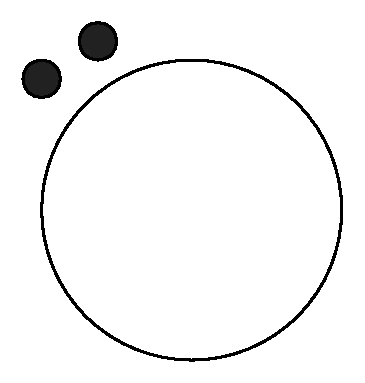
\includegraphics[width=.2\linewidth]{lm/table_2} &
	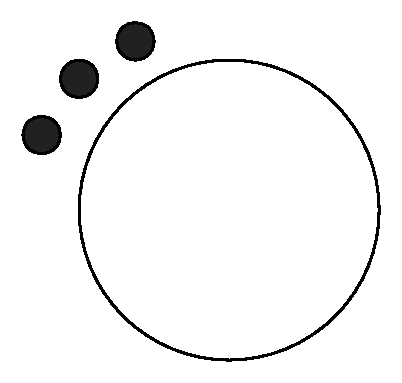
\includegraphics[width=.2\linewidth]{lm/table_3} &
	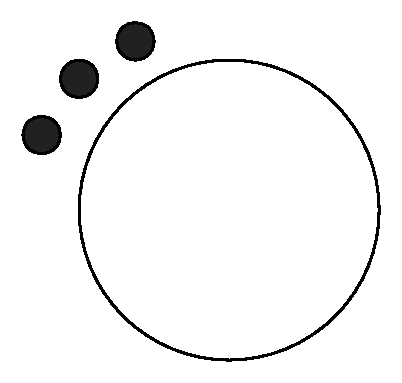
\includegraphics[width=.2\linewidth]{lm/table_3} &
         
\includegraphics[width=.2\linewidth]{lm/table_0} \\
	 \pause
	 $\frac{2}{7 + \alpha}$ & $\frac{3}{7 + \alpha}$ & $\frac{2}{7 + \alpha}$ & $\frac{\alpha}{7 + \alpha}$ \\
	 \pause
	 dog & cat & purple & \alert<4>{???} \\
	\end{tabular}
	\end{center}


\end{frame}


\begin{frame}{What to do with a new table?}

  \gfx{crp_new_table}{.8}

\pause
\begin{block}{What can be a base distribution?}
\begin{itemize}
  \item Uniform (Dirichlet smoothing)
\pause
  \item Specific contexts $\rightarrow$ less-specific contexts (backoff)
\end{itemize}
\end{block}

\end{frame}


\begin{frame}{A hierarchy of Chinese Restaurants}

  \gfx{prefixes}{.9}

\end{frame}


\begin{frame}{Seating Assignments}
{\bf Dataset:} \texttt{\alert<2-5>{<s>} \alert<2-5,6-8>{a} \alert<6-8,9-10>{a} \alert<9-10,11-14>{a}
  \alert<11-14,15-18>{b} \alert<15-18,19-22>{a} \alert<19-22,23-26>{c} \alert<23-26>{</s>}}

\pause

% <s> a 2-5
% a a 6-8
% a a 9-10
% a b 11-14
% b a 15-18
% a c 19-22
% c </s> 23-26


\begin{block}{Unigram Restaurant}
       \only<5-7>{\alert<7>{\mymk{a}{1}}}
       \only<8-17>{\alert<17>{\mymk{a}{2}}}
       \only<18->{\mymk{a}{3}}
       \only<13->{\alert<13>{\mymk{b}{1}}}
       \only<22->{\alert<22>{\mymk{c}{1}}}
       \only<26->{\alert<26>{\mymk{</s>}{1}}}
       \only<4,12,21,25>{\mymk{*}{1}}
\end{block}

\begin{columns}
  \column{.45\linewidth}
     \begin{block}{\texttt{<s>} Restaurant}
       \only<3-4>{\mymk{*}{1}}
        \only<5->{\mymk{a}{1}}
     \end{block}

     \begin{block}{\texttt{b} Restaurant}
        \only<18->{\mymk{a}{1}}
       \only<16-17>{\mymk{*}{1}}
     \end{block}

  \column{.45\linewidth}
     \begin{block}{\texttt{a} Restaurant}
       \only<8-9>{\mymk{a}{1}}
        \only<10->{\mymk{a}{\alert<10>{2}}}
        \only<14->{\mymk{b}{1}}
        \only<22->{\mymk{c}{1}}
        \only<6-7,11-13,20-21>{\mymk{*}{1}}
     \end{block}

     \begin{block}{\texttt{c} Restaurant}
        \only<26->{\mymk{</s>}{1}}
       \only<24-25>{\mymk{*}{1}}
     \end{block}


\end{columns}

\end{frame}

\begin{frame}{Real examples}

	\begin{itemize}
		\item San Francisco
		\pause
		\item Star Spangled Banner
		\pause
		\item Bottom Line: Counts go to the context that explains it best
	\end{itemize}

\end{frame}


\begin{frame}{The rich get richer}

	\begin{center}
	\begin{tabular}{ccc}
	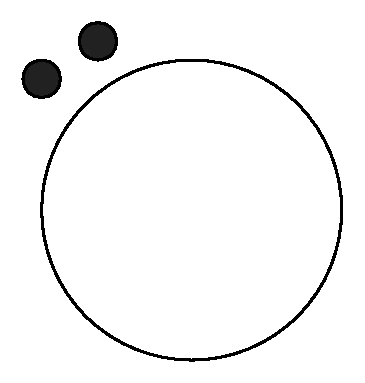
\includegraphics[width=.2\linewidth]{lm/table_2} &
	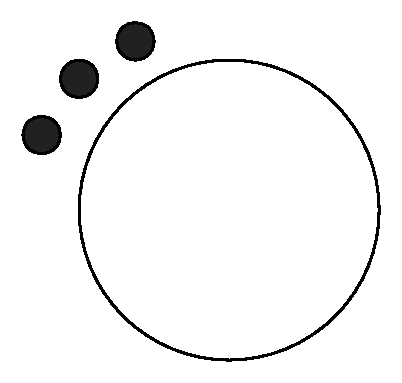
\includegraphics[width=.2\linewidth]{lm/table_3} &
	
\includegraphics[width=.2\linewidth]{lm/table_0} \\
	 $\frac{2}{5+\theta}$ & $\frac{3}{5 + \theta}$ & $\frac{\theta}{5+\theta}$ \\
	\end{tabular}
	\end{center}


\end{frame}

\begin{frame}{Computing the Probability of an Observation}

\begin{equation}
   p(w=\alert<1>{x} | \alert<2>{\vec{s}}, \alert<3>{\theta},
   \alert<4>{u}) = \explain{existing table}{\frac{\alert<5>{c_{u,x}}}{\theta + \alert<6>{c_{u,\cdot}}}}
   + \explain{new table}{\frac{\alert<3>{\theta}}{\theta + c_{u, \cdot}} p(w=x | \vec{s}, \theta, \alert<7>{\pi(\alert<4>{u})})}
\end{equation}

\begin{itemize}
  \item Word type $\alert<1>{x}$
  \item Seating assignments $\alert<2>{\vec{s}}$
  \item Concentration $\alert<3>{\theta}$
  \item Context $\alert<4>{u}$
  \item Number seated at table serving $x$ in restaurant $u$, $\alert<5>{c_{u,x}}$
  \item Number seated at all tables in restaurant $u$, $\alert<6>{c_{u,\cdot}}$
  \item The backoff context $\alert<7>{\pi(u)}$

\end{itemize}

\end{frame}




\begin{frame}{Example: $p(w=\texttt{b} | \vec{s}, \theta=1.0, u=\texttt{a})$}


\begin{block}{Unigram Restaurant}
  \mymk{a}{3}
  \mymk{b}{1}
  \mymk{c}{1}
  \mymk{</s>}{1}
\end{block}

\begin{columns}
  \column{.45\linewidth}
     \begin{block}{\texttt{<s>} Restaurant}
       \mymk{a}{1}
     \end{block}

     \begin{block}{\texttt{b} Restaurant}
        \mymk{a}{1}
     \end{block}

  \column{.45\linewidth}
     \begin{block}{\texttt{a} Restaurant}
       \mymk{a}{2}
       \mymk{b}{1}
        \mymk{c}{1}
     \end{block}

     \begin{block}{\texttt{c} Restaurant}
         \mymk{</s>}{1}
     \end{block}

\end{columns}

\begin{equation}
   p(w=\texttt{b} | \dots ) =
\only<-8>{
   \frac{\only<-2>{c_{\texttt{a},\texttt{b}}}
     \only<3->{1}}{\only<-3>{\theta} \only<4->{1.0} +
     \only<-4>{c_{u,\cdot}} \only<5->{4}}
   +
   \frac{\only<-3>{\theta}\only<4->{1.0}}{\only<-3>{\theta}\only<4->{1.0}
     + \only<-4>{c_{u, \cdot}}\only<5->{4}} \alert<6>{p(w=x | \vec{s},
     \theta, \pi(\only<-6>{u}\only<7->{\emptyset}))}
}
\only<9-13>{
  \frac{1}{5} + \frac{1}{5} \left(
    \frac{\only<-11>{c_{\emptyset,\texttt{b}}}\only<12->{1}}{\only<-12>{c_{\emptyset, \cdot}}\only<13->{6} + \only<-10>{\theta}\only<11->{1.0}} +
    \frac{\only<-10>{\theta}\only<11->{1.0}}{\only<-12>{c_{\emptyset, \cdot}}\only<13->{6}  + \only<-10>{\theta}\only<11->{1.0}} \alert<9>{\frac{1}{\only<-9>{V}\only<10->{5}}} \right)
}
\only<14>{
\frac{1}{5} + \frac{1}{5}\left(\frac{1}{7} +
  \frac{1}{7}\frac{1}{5}\right) = 0.24
}
\end{equation}

\end{frame}

\begin{frame}{Discounting}

\begin{itemize}
  \item Empirically, it helps favor the backoff if you have more
    tables
  \item Otherwise, it gets too close to maximum likelihood
  \item Idea is called \emph{discounting}
  \item Steal a little bit of probability mass $\delta$ from every table and
    give it to the new table (backoff)
\end{itemize}
\pause

\begin{equation}
   p(w=x | \vec{s}, \theta, u) = \explain{existing
     table}{\frac{c_{u,x} \only<3->{- \alert<3>{\delta}}}{\theta + c_{u,\cdot}}}
   + \explain{new table}{\frac{\theta \only<3->{+ \alert<4>{T}\alert<3>{\delta}}}{\theta + c_{u, \cdot}} p(w=x | \vec{s}, \theta, \pi(u))}
\end{equation}

\only<5->{{\bf Interpolated Kneser-Ney!}}

\end{frame}

\begin{frame}{More advanced models}

\begin{itemize}
  \item Interpolated Kneser-Ney assumes {\bf one table with a dish
      (word)} per restaurant (known as {\bf minimal} path assumption)
  \item Can get slightly better performance by assuming you can have
    duplicated tables: {\bf Pitman-Yor} language model
  \item Requires Gibbs Sampling of the seating assignments
    \begin{itemize}
      \item Initialize seating assignments
      \item Remove word from context
      \item Add it back in (seating probabilistically)
    \end{itemize}
\end{itemize}

\end{frame}

\begin{frame}{Exercise}
  \begin{itemize}
    \item Start with restaurant we had before
    \item Assume you see \texttt{<s> b b a c </s>}; add those counts
      to tables
    \item Compute probability of \texttt{b} following \texttt{a}
      ($\theta=1.0, \delta=0.5$)
    \item Compute the probability of \texttt{a} following \texttt{b}
    \item Compute probability of \texttt{</s>} following \texttt{<s>}
  \end{itemize}

\end{frame}

\begin{frame}{A busy night at the restaurant}


\begin{block}{Unigram Restaurant}
  \mymk{a}{3}
  \only<-2>{\mymk{b}{1}}
  \only<3-4>{\alert<3>{\mymk{b}{2}}}
  \only<5->{\alert<5>{\mymk{b}{3}}}
  \mymk{c}{1}
  \mymk{</s>}{1}
\end{block}

\begin{columns}
  \column{.45\linewidth}
     \begin{block}{\texttt{<s>} Restaurant}
       \mymk{a}{1}
       \only<2->{\alert<2>{\mymk{b}{1}}}
     \end{block}

     \begin{block}{\texttt{b} Restaurant}
	\only<-5>{\mymk{a}{1}}
	\only<6->{\alert<6>{\mymk{a}{2}}	}
        \only<4->{	\alert<4>{\mymk{b}{1}}}

     \end{block}

  \column{.45\linewidth}
     \begin{block}{\texttt{a} Restaurant}
       \mymk{a}{2}
       \mymk{b}{1}
        \only<-6>{\mymk{c}{1}}
        \only<7->{\alert<7>{\mymk{c}{2}}        }
     \end{block}

     \begin{block}{\texttt{c} Restaurant}
         \only<-7>{\mymk{</s>}{1}}
         \only<8->{\alert<8>{\mymk{</s>}{2}}  }
     \end{block}

\end{columns}

\only<9->{As you see more data, bottom restaurants do more work.}

\end{frame}

\begin{frame}{\texttt{b} following \texttt{a}}

	\begin{align}
	=\frac{1 - \delta}{\theta + 5} + \frac{\theta + 3\delta}{\theta + 5} & p(\mbox{\texttt{b}}) \\
	\pause
	=\frac{1 - \delta}{\theta + 5} + \frac{\theta + 3\delta}{\theta + 5} & \left(\frac{3 - \delta}{\theta + 8} + \frac{\theta + 4\delta}{\theta + 8}\frac{1}{V} \right) \\
	\end{align}

\begin{center}
	\only<3->{0.23}
\end{center}

\end{frame}

\begin{frame}{\texttt{a} following \texttt{b}}

	\begin{align}
	=\frac{2 - \delta}{\theta + 3} + \frac{\theta + 2\delta}{\theta + 3} & p(\mbox{\texttt{a}}) \\
	\pause
	=\frac{2 - \delta}{\theta + 3} + \frac{\theta + 2\delta}{\theta + 3} & \left(\frac{3 - \delta}{\theta + 8} + \frac{\theta + 4\delta}{\theta + 8}\frac{1}{V} \right) \\
	\end{align}

\begin{center}
	\only<3->{0.55}
\end{center}

\end{frame}


\begin{frame}{\texttt{</s>} following \texttt{<s>}}

	\begin{align}
	=\frac{\theta + 2\delta}{\theta + 2} & p(\mbox{\texttt{</s>}}) \\
	\pause
	=\frac{\theta + 2\delta}{\theta + 2} & \left(\frac{1 - \delta}{\theta + 8} + \frac{\theta + 4\delta}{\theta + 8}\frac{1}{V} \right) \\
	\end{align}

\begin{center}
	\only<3->{0.08}
\end{center}

\end{frame}


\end{document}
